%%%%%%%%%%%%%%%%%%%%%%%%%%%%%%%%%%%%%%%%%
% Beamer Presentation
% LaTeX Template
% Version 1.0 (10/11/12)
%
% This template has been downloaded from:
% http://www.LaTeXTemplates.com
%
% License:
% CC BY-NC-SA 3.0 (http://creativecommons.org/licenses/by-nc-sa/3.0/)
%
%%%%%%%%%%%%%%%%%%%%%%%%%%%%%%%%%%%%%%%%% 

%----------------------------------------------------------------------------------------
%   PACKAGES AND THEMES
%----------------------------------------------------------------------------------------

\documentclass[xcolor=dvipsnames]{beamer}
\usepackage{graphicx} % Allows including images
\usepackage{tikz}
\usepackage{pgfplots}
\usepackage{pgf}
\usepackage{soul}
%\usepackage{hyperref}
\pgfplotsset{compat=newest}

%\usepackage{amsmath} % Add amssymb if not using Mathtime
\newcommand\numberthis{\addtocounter{equation}{1}\tag{\theequation}}

% Set arrow type
\input{/Users/mqwilber/Dropbox/Documents/Latex/arrowsnew}
\usetikzlibrary{arrows,shapes,backgrounds}
\tikzset{>=latex}

%\usefonttheme{professionalfonts}
\usepackage{fontspec}
\setsansfont[UprightFont={* Light},
             BoldFont={* SemiBold},
             ItalicFont={* Light Italic},
             BoldItalicFont={* SemiBold Italic}]{Gill Sans}

%\setsansfont[UprightFont={* Light}]{Helvetica}
%\setsansfont{Papyrus}
% \setsansfont[Path = /usr/local/texlive/2014/texmf-dist/fonts/truetype/huerta/alegreya/,
% Extension=.ttf
% ]{AlegreyaSC-Regular}

% Set graphics path
\graphicspath{{images/}}


\renewcommand\footnoterule{}
\newcommand{\tc}{\textcolor{red}}
\newcommand{\tb}{\textcolor{blue}}
\newcommand\ig[1]{\includegraphics[width=#1\textwidth]}

\definecolor{dgreen}{rgb}{0.,0.6,0.}
\setbeamertemplate{caption}{\raggedright\insertcaption\par}
% \usepackage[dvipsnames]{xcolor}

% Color of frame title
\setbeamercolor{frametitle}{fg=Black, bg=White}
\setbeamertemplate{frametitle}[two lines]

% Change color of title
\setbeamercolor{title}{fg=Black, bg=White}

% Change color of enumerated list
\setbeamertemplate{enumerate item}{\color{Black}\insertenumlabel.}

\setbeamertemplate{itemize item}{\color{Black}\tikz[baseline=-0.8ex]\draw[black,fill=black] (0,0) circle (.3ex);}
\setbeamertemplate{itemize subitem}{\color{Black}\tikz[baseline=-0.8ex]\draw[black,fill=black] (0,0) circle (.2ex);}

%% Personal commands

% Define frog
\def\cfrog{\includegraphics[width=0.8cm]{/Users/mqwilber/Repos/completed_projects/empirical_taylor_law/docs/presentation/images/frog_sw}}

\def\cfrognew{\includegraphics[width=.15\textwidth]{/Users/mqwilber/Repos/completed_projects/density_dependent_ipm/docs/presentation/images/cfrog}}
\def\cinfrognew{\includegraphics[width=.15\textwidth]{/Users/mqwilber/Repos/completed_projects/density_dependent_ipm/docs/presentation/images/infected_cfrog}}

\def\border{draw, ultra thick, inner sep=.8}

\newcommand{\numfrog}[1]
{   \begin{tikzpicture}
      \node[opacity=0.5] at (0, 0) (frog) {\includegraphics[width=1.4cm]{/Users/mqwilber/Repos/completed_projects/empirical_taylor_law/docs/presentation/images/frog_sw}};
      \node[inner sep=0.8, draw, fill=white] at (0, 0) {\textcolor{black}{#1}};
    \end{tikzpicture}
}

% Footnote without a marker
\newcommand\blfootnote[1]{%
  \begingroup
  \renewcommand\thefootnote{}\footnote{#1}%
  \addtocounter{footnote}{-1}%
  \endgroup
}

\mode<presentation> {

% The Beamer class comes with a number of default slide themes
% which change the colors and layouts of slides. Below this is a list
% of all the themes, uncomment each in turn to see what they look like.

\usetheme{default}
%\usetheme{AnnArbor}
%\usetheme{Antibes}
%\usetheme{Bergen}
%\usetheme{Berkeley}
%\usetheme{Berlin}
%\usetheme{Boadilla}
%\usetheme{CambridgeUS}
%\usetheme{Copenhagen}
%\usetheme{Darmstadt}
%\usetheme{Dresden}
%\usetheme{Frankfurt}
%\usetheme{Goettingen}
%\usetheme{Hannover}
%\usetheme{Ilmenau}
%\usetheme{JuanLesPins}
%\usetheme{Luebeck}
%\usetheme{Madrid}
%\usetheme{Malmoe}
%\usetheme{Marburg}
%\usetheme{Montpellier}
%\usetheme{PaloAlto}
%\usetheme{Pittsburgh}
%\usetheme{Rochester}
%\usetheme{Singapore}
%\usetheme{Szeged}
%\usetheme{Warsaw}

% As well as themes, the Beamer class has a number of color themes
% for any slide theme. Uncomment each of these in turn to see how it
% changes the colors of your current slide theme.

%\usecolortheme{albatross}
%\usecolortheme{beaver}
%\usecolortheme{beetle}
%\usecolortheme{crane}
%\usecolortheme{dolphin}
%\usecolortheme{dove}
%\usecolortheme{fly}
%\usecolortheme{lily}
%\usecolortheme{orchid}
%\usecolortheme{rose}
%\usecolortheme{seagull}
%\usecolortheme{seahorse}
%\usecolortheme{whale}
%\usecolortheme{wolverine}

\setbeamertemplate{footline} % To remove the footer line in all slides uncomment this line
%\setbeamertemplate{footline}[page number] % To replace the footer line in all slides with a simple slide count uncomment this line

\setbeamertemplate{navigation symbols}{} % To remove the navigation symbols from the bottom of all slides uncomment this line
}


% Centers the frametitles of each slide
% \setbeameroption{show notes}
\setbeamertemplate{frametitle}[default][center]

% Adding

\title{RSFs and feral swine movement} % The
% short
% title appears at the bottom
% of every
% slide, the full title is only on the title page

\author{CSU lab meeting}
\institute[CSU]
{
\smallskip

}
\date{April 4, 2018} % Date, can be changed to a custom date

%\titlegraphic{\includegraphics[scale=0.25]{example_tpl.png}}

\begin{document}

% Remember pictures
\tikzstyle{every picture}+=[remember picture]
\tikzstyle{na} = [baseline=-.5ex]

\begin{frame}
\titlepage % Print the title page as the first slide
\end{frame}


%------------------------------------------------

\begin{frame}[t]
\frametitle{\underline{A tiny bit about feral swine}}
  
  \begin{enumerate}
    \item<1-> Endemic in the Southeast and California and spreading northward
    \item<2-> Limited by water availability and temperature/snow cover
    \item<3-> Eat just about anything
  \end{enumerate}

  \only<1>{
  \centering
  \ig{0.7}{images/snow.png}
  \blfootnote{\hfill \tiny Snow et al. 2017}
  }
  \only<2>{
    \centering
    \vfill
    \ig{0.7}{images/wallow.pdf}
  }
  \only<3-4>{

    \centering
    \only<3>{\ig{0.5}{cropdamage.pdf}}
    \only<4>{\ig{0.7}{images/wildpigdeer.pdf}}
  }
  
\end{frame}

%------------------------------------------------

\begin{frame}[t]
\frametitle{\underline{Original questions}}
  
  \begin{enumerate}
    \item<1-> What factors drive feral swine resource selection and how does this change across a latitudinal and longitudinal gradient? 
      \begin{itemize}
        \item<2-> Really broad and kind of vague
      \end{itemize}

    \item<3-> How does the availability of natural forage resources and anthropogenic forage resources on a landscape affect pig movement? 

    \item<4> How does the availability of natural forage resources affect how pig's use anthropogenic forage resources?

  \end{enumerate}

\end{frame}

%------------------------------------------------

% \begin{frame}[t]
% \frametitle{\underline{The data}}
  
%   \only<1>{
%   \centering
%   \begin{tikzpicture}
  
%     \node at (0, 0) {\ig{1}{datamap.pdf}};
%     \node[align=center] at (4, -2) {500 pigs \\ 36 studies};

%   \end{tikzpicture}}

%   \only<2>{
%     118 of the 207 currently processed pigs have ``used'' crops as a resource 

%     \ig{0.9}{/Users/mqwilber/Repos/rsf_swine/results/crop_use_overall.pdf}
%   }


% \end{frame}

%------------------------------------------------

\begin{frame}[t]
\frametitle{\underline{The data}}
  
  \centering
  \begin{tikzpicture}
  
    \node at (0, 0) {\ig{1}{datamap.pdf}};
    \node[align=center] at (4, -2) {500 pigs \\ 36 studies};

    \node<2>[draw, minimum width=0.5cm, minimum height=0.5cm, red, ultra thick] at (-3.6, -1) {};
  \end{tikzpicture}
  
\end{frame}

%------------------------------------------------

\begin{frame}[t]
\frametitle{\underline{Linking resource selection with movement data: Tejon, CA}}
  
  \only<1-3>{
  \centering 
  How does pig movement reflect resource selection and vice versa?}

  \only<2>{
  \begin{itemize}
    \item 13 pigs: 8 female and 7 male
  \end{itemize}

  \ig{0.8}{tejonmovement}
  }

  \only<3>{
    
    \ig{1}{mastingplot.jpg}
  }

  \only<4-7>{


    \centering
    In a time step, given all of the locations that are available, what does a pig ``use''?

    \only<5>{
    \ig{0.7}{Northrup.png}
    \blfootnote{\hfill \tiny Northrup et al. 2016}
    }

    \only<6-7>{
      \begin{equation}
        [\text{resources} | \text{use}] = \frac{[\text{use} | \text{resources}] [\text{resources}]}{[\text{use}]}
      \end{equation}

      \begin{itemize}
        \item $[\text{use} | \text{resources}]$: Resource utilization function (what we want)
        \item $[\text{resources}]$: Available resources
      \end{itemize}

      \only<7>{

        \bigskip
        \flushleft

        To model pig selection for forage resource we need to
        \begin{enumerate}
          \item Identify covariate proxies for ``resource''
          \item Identify ``available'' habitat
        \end{enumerate}
      }
    }


  }

\end{frame}

%------------------------------------------------

\begin{frame}[t]
\frametitle{\underline{Covariates for pig resource selection}}
  

  
  \begin{columns}
    \begin{column}{0.5\textwidth}
      Non-foraging resources (at least not directly)

      \begin{itemize}
        \item Water availability
        \item Tree cover
        \item Temperature
        \item Precipitation
        \item Snow depth
        \item Elevation
        \item Human development index
      \end{itemize}
       
    \end{column}
    \begin{column}{0.5\textwidth}
      Foraging resources

      \begin{itemize}
        \item Crop availability (Anthropogenic forage)
        \item Livestock presence (Anthropogenic forage)
        \item Plant productivity (Natural forage)
        \item Masting tree density (Natural forage)
      \end{itemize}
    
    \end{column}
  \end{columns}

  \only<2>{
  \bigskip
  \centering
  How do foraging resources drive pig resource selection, after accounting for non-foraging resources?}

\end{frame}

%------------------------------------------------


\begin{frame}[t]
\frametitle{\underline{Identify ``available'' habitat with movement model}}

  \underline{Step 1:} Fit a continuous-time movement model to GPS data

    \only<1>{
    \centering
    \ig{0.9}{tejonpath.pdf}
    }
    \only<2>{
    \centering
    \ig{0.9}{tejonpath_pred.pdf}
    }

    \blfootnote{\hfill \tiny Buderman et al. 2016}
    

\end{frame}

%------------------------------------------------



\begin{frame}[t]
\frametitle{\underline{Identify ``available'' habitat with movement model}}

  \underline{Step 2:} Convert continuous path into discrete environmental space 

  \centering
  \ig{0.55}{hooten.png}

  Yields a continuous-time, discrete-state movement model. 
  
  \blfootnote{\hfill \tiny Hooten et al. 2010, Hanks et al. 2015, Buderman et al. 2018}

\end{frame}

%------------------------------------------------

\begin{frame}[t]
\frametitle{\underline{Predict resource utilization}}
  
  Covariates + movement model $\rightarrow$ prediction of resource utilization

  \begin{enumerate}
    \item \emph{Location-based covariates}: How long a pig remains in a cell as a function of resource

    \item \emph{Directional covariates}: The direction in which a pig moves from that cell as a function of the resource gradient
  \end{enumerate} 

  \bigskip
  \centering
  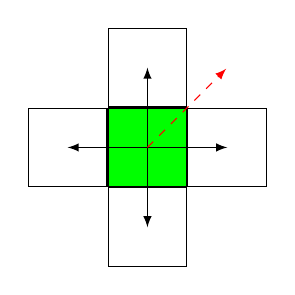
\begin{tikzpicture}
    \node[draw, minimum height=1cm, minimum width=1cm, fill=green] at (0,  0) (mid) {};
    \node[at=(mid.south), below, draw, minimum height=1cm, minimum width=1cm] (down) {};
    \node[at=(mid.north), above, draw, minimum height=1cm, minimum width=1cm] (up) {};
    \node[at=(mid.east), right, draw, minimum height=1cm, minimum width=1cm] (right) {};
    \node[at=(mid.west), left, draw, minimum height=1cm, minimum width=1cm] (left) {};

    \only<2->{
    \draw[->] (mid.center)--(down.center);
    \draw[->] (mid.center)--(up.center);
    \draw[->] (mid.center)--(right.center);
    \draw[->] (mid.center)--(left.center);


    \draw[->, dashed, red] (mid.center)--(1, 1);}
  \end{tikzpicture}

  \only<3>{
  \begin{equation*}
    \log \lambda_{ij} = \log{\tau_{ij}} + \beta \mathbf{X} \text{ where \textbf{X} contains location and directional covariates}
  \end{equation*}
  }

\end{frame}




%------------------------------------------------

\begin{frame}[t]
\frametitle{\underline{An example from Tejon}}

  Spatial scale: 30m by 30m

  \only<1>{\ig{1}{tejonlayers.pdf}}
  \only<2>{\ig{1}{tejonlayers_wpig.pdf}}

  \bigskip
  \only<3>{
    Fruit and nuts drive the direction of this pig's movement

    \ig{0.95}{fruitnutgrad.pdf}
  }
  \only<4>{
    Pig spends more time in increased canopy during mid-day

    \ig{0.95}{canopycoverloc.pdf}
  }

\end{frame}

%------------------------------------------------

\begin{frame}[t]
\frametitle{\underline{Where we are trying to go...and some challenges}}

How does the availability of natural forage resources and anthropogenic forage resources affect pig movement on a landscape?

\begin{itemize}
  \item<1-> Are there any consistent effects of forage resource use across pigs/populations?
    \begin{itemize}
      \item Currently performing movement analyses across populations. Summary: its a mess.
      \item Not all pigs use crops. Just focus on crop-users? 
    \end{itemize}
  \item<2-> Selection of foraging resources changes seasonally
    \begin{itemize}
      \item Does the ``pull'' of crops depend on the availability of natural resource?
    \end{itemize}
  \item<3-> Spatial scale affects resource selection
  \begin{itemize}
    \item At what scale does a pig select a particular resource?
  \end{itemize}
\end{itemize}

\end{frame}


\end{document}

